\documentclass[aspectratio=169,10pt]{beamer}
\usetheme{Madrid}
\usepackage[T1]{fontenc}

\usepackage{fancybox,graphicx,hyperref,url}
\usepackage{tikz}
\usetikzlibrary{shapes,arrows}
\usetikzlibrary{positioning}
\usepackage{booktabs}
\usepackage{enumitem}

\usepackage{listings}
\usepackage{lstautogobble}
\input{lstisabelle}
\usepackage[listings,skins,breakable,xparse]{tcolorbox}
\tcbuselibrary{theorems}
\tcbset{highlight math/.append style={boxrule=0pt,
                                      frame hidden,
                                      colback=yellow!40!white,
                                      sharp corners}}

\usepackage{xpatch}
\usepackage{xcolor}
\usepackage{realboxes}

\makeatletter
\xpretocmd\lstinline{\Colorbox{yellow!10!white}\bgroup\appto\lst@DeInit{\egroup}}{}{}
\makeatother

\definecolor{my_red}{RGB}{128, 0, 0}

\lstset{captionpos=b}
\lstset{numberbychapter=false}
\lstset{autogobble}
% \lstset{breaklines=true}

\usepackage{tikz}
\usepackage{subcaption}
\usetikzlibrary{calc, chains, decorations.pathmorphing}
\usetikzlibrary{shapes,arrows,backgrounds}
\usetikzlibrary{positioning,fit,shapes.geometric,shapes}

\setbeamercovered{transparent}

\setlistdepth{9}
\setlist[itemize,1]{label=$\bullet$}
\setlist[itemize,2]{label=$\bullet$}
\setlist[itemize,3]{label=$\bullet$}
\setlist[itemize,4]{label=$\bullet$}
\setlist[itemize,5]{label=$\bullet$}
\setlist[itemize,6]{label=$\bullet$}
\setlist[itemize,7]{label=$\bullet$}
\setlist[itemize,8]{label=$\bullet$}
\setlist[itemize,9]{label=$\bullet$}
\renewlist{itemize}{itemize}{9}

\setlist[enumerate,1]{label=$\arabic*.$}
\setlist[enumerate,2]{label=$\alph*.$}
\setlist[enumerate,3]{label=$\roman*.$}
\setlist[enumerate,4]{label=$\arabic*.$}
\setlist[enumerate,5]{label=$\alpha*$}
\setlist[enumerate,6]{label=$\roman*.$}
\setlist[enumerate,7]{label=$\arabic*.$}
\setlist[enumerate,8]{label=$\alph*.$}
\setlist[enumerate,9]{label=$\roman*.$}
\renewlist{enumerate}{enumerate}{9}

\AtBeginSection[]{
  \begin{frame}[noframenumbering]
    \vfill
    \centering
    \begin{beamercolorbox}[sep=8pt,center,shadow=true,rounded=true]{title}
      \usebeamerfont{title}\insertsectionhead\par%
    \end{beamercolorbox}
    \vfill
  \end{frame}
}

\title[Verified Time-Aware Stream Processing]{Verified Time-Aware Stream Processing}

\author[Rafael Castro]{
  Rafael Castro G. Silva\\\medskip
  {\small \url{rasi@di.ku.dk}}}

\date{02/11/2023}

\institute[UCPH]{
  Department of Computer Science \\
  University of Copenhagen}

\begin{document}

\begin{frame}
  \titlepage

\end{frame}

\begin{frame}[fragile]
  \frametitle{What is this PhD/Status seminar about?}
  \begin{itemize}
    \item Distributed Systems
          \begin{itemize}
            \item Stream processing frameworks
                  \begin{itemize}
                    \item Dataflow models
                          \begin{itemize}
                            \item Time-Aware Computations
                          \end{itemize}
                  \end{itemize}
          \end{itemize}
    \item Formal Methods
          \begin{itemize}
            \item Verification using proof assistants
                  \begin{itemize}
                    \item Isabelle proofs
                          \begin{itemize}
                            \item Verified and executable code
                          \end{itemize}
                  \end{itemize}
          \end{itemize}
    \item Formalization of Time-Aware Stream Processing
  \end{itemize}
\end{frame}

\begin{frame}{Contents}
  \begin{itemize}
    \item Introduction
    \item Preliminaries
    \item Lazy Lists Processors
    \item Time-Aware Operators
    \item Case Study
    \item Next Steps
  \end{itemize}
\end{frame}

\section{Introduction}

\begin{frame}[fragile]
  \frametitle{Dataflow Models}
  \begin{itemize}
    \item Stream Processing
    \item Dataflow Model
    \item Time-Aware Computations
    \item Bugs in Stream Processing
  \end{itemize}
\end{frame}

\section{Preliminaries}
\begin{frame}[fragile]
  \frametitle{Isabelle/HOL}
  \begin{itemize}
    \item HOL
    \item Isabelle/HOL
  \end{itemize}
\end{frame}

\begin{frame}[fragile]
  \frametitle{Isabelle/HOL: (Co)datatypes}
  \begin{itemize}
    \item Datatypes and Codatatypes
          \begin{tcblisting}{hbox,listing only,listing options={language=isabelle,aboveskip=0pt,belowskip=0pt},size=fbox,boxrule=0pt,frame hidden,arc=0pt,colback=yellow!10!white}
codatatype (lset: 'a) llist = lnull: LNil | LCons (lhd: 'a) (ltl: "'a llist")
  for map: lmap where "ltl LNil = LNil"
          \end{tcblisting}

    \item Induction principle for \is{lset} membership:
  \begin{tcolorbox}[ams align,colback=yellow!10!white,colframe=my_red, top=0pt, arc=0pt, size=fbox,boxrule=1pt]
    \begin{array}{@{}l@{}}
      \text{\is{x \\in lset lxs --> (!! x lxs. P x (LCons x lxs)) -->}}
      \\
      \text{\is{(!!x lxs y . y \\in lset lxs --> P y lxs --> P y (LCons x lxs)) -->> P x lxs}}
    \end{array}
  \end{tcolorbox}

    \item Coinductive principle for lazy list equality:
          \begin{itemize}
            \item Show a \emph{bisimulation} \is{R} that relates the lazy lists:
\begin{tcolorbox}[ams align,colback=yellow!10!white,colframe=my_red, top=0pt, arc=0pt, size=fbox,boxrule=1pt]
  \hspace*{-0.7cm}
  \begin{array}{@{}l@{}}
  \text{\is{R lxs lys --> !!lxs lys . R lxs lys --> lnull lxs <--> lnull lys \\and}}
  \\
  \quad\text{\is{\\<not>lnull lxs --> \\<not>lnull lys --> lhd lxs = lhd lys \\and R (ltl lxs) (ltl lys)) -->> lxs = lys}}
  \end{array}
\end{tcolorbox}
          \end{itemize}
  \end{itemize}
\end{frame}

\begin{frame}[fragile]
  \frametitle{Isabelle/HOL: Recursion and While Combinator}
  \begin{itemize}
    \item Recursion

\begin{tcblisting}{hbox,listing only,listing options={language=isabelle,aboveskip=0pt,belowskip=0pt},size=fbox,boxrule=0pt,frame hidden,arc=0pt,colback=yellow!10!white}
fun lshift :: "'a list => 'a llist => 'a llist" (infixr @@ 65) where
  "lshift [] lxs = lxs"
| "lshift (x # xs) lxs = LCons x (lshift xs lxs)"
\end{tcblisting}
  \item While Combinator
\begin{tcblisting}{hbox,listing only,listing options={language=isabelle,aboveskip=0pt,belowskip=0pt},size=fbox,boxrule=0pt,frame hidden,arc=0pt,colback=yellow!10!white}
definition while_option :: "('a => bool) => ('a => 'a) => 'a => 'a option" where
"while_option b c s = (if (?k. \<not> b ((c ^^ k) s))
   then Some ((c ^^ (LEAST k. \<not> b ((c ^^ k) s))) s)
   else None)"
\end{tcblisting}
    \item While rule
\begin{tcolorbox}[ams align,colback=yellow!10!white,colframe=my_red, top=0pt, arc=0pt, size=fbox,boxrule=1pt]\label{while_option_rule}
  \begin{array}{@{}l@{}}
    \text{{\is{Q s --> while_option t b s = Some s' --> (!!s. Q s --> t s --> Q (b s)) -->> Q s'}}}
  \end{array}
\end{tcolorbox}
          \end{itemize}
\end{frame}

\begin{frame}[fragile]
  \frametitle{Isabelle/HOL: Corecursion and Friends}
  \begin{itemize}
    \item Corec
    \item Friend
  \end{itemize}
\end{frame}

\begin{frame}[fragile]
  \frametitle{Isabelle/HOL: (Co)inductive Predicates}
  \begin{itemize}
    \item Inductive
    \item Coinductive
    \item Coinduction
  \end{itemize}

\end{frame}

\section{Lazy Lists Processors}

\begin{frame}[fragile]
  \frametitle{Operators}
  \begin{itemize}
    \item Operator
    \item Produce \lstinline{produce}
    \item Example
  \end{itemize}

  \begin{figure}[!t]
    \begin{subfigure}{.5\textwidth}
      \raggedright
      \begin{tabular}{@{}l@{}}
        \text{\is{stream_1 =}}
        \\
        \begin{tikzpicture}[scale=0.9, every node/.style={scale=0.9},background rectangle/.style={fill=yellow!10!white},show background rectangle]
          \tikzset{tape/.style={minimum size=.6cm, draw}}
          \begin{scope}[start chain=0 going right, node distance=0mm]
            \foreach \x [count=\i] in {\is{DT t_4 **d**},\is{DT t_0 **a**},\is{DT t_1 **c**},\is{WM t_1},\is{DT t_5 **c**}} {
              \ifnum\i=5
                \node [on chain=0, tape, outer sep=0pt] (n\i) {\x};
                \draw (n\i.north east) -- ++(.1,0) decorate [decoration={zigzag, segment length=.12cm, amplitude=.02cm}] {-- ($(n\i.south east)+(+.1,0)$)} -- (n\i.south east) -- cycle;
              \else
                \node [on chain=0, tape] (n\i) {\x};
              \fi
            }
          \end{scope}
        \end{tikzpicture}
        \vspace*{-1.3ex}
        \\
        \begin{tikzpicture}[scale=0.9, every node/.style={scale=0.9},background rectangle/.style={fill=yellow!10!white},show background rectangle]
          \tikzset{tape/.style={minimum size=.6cm, draw}}
          \begin{scope}[start chain=0 going right, node distance=0mm]
            \foreach \x [count=\i] in {\is{DT t_3 **a**},\is{DT t_5 **a**},\is{WM t_2},\is{WM t_5},\is{DT t_2 **b**}} {
              \ifnum\i=5
                \node [on chain=0, tape, outer sep=0pt] (n\i) {\x};
                \draw (n\i.north east) -- ++(.1,0) decorate [decoration={zigzag, segment length=.12cm, amplitude=.02cm}] {-- ($(n\i.south east)+(+.1,0)$)} -- (n\i.south east) -- cycle;
              \else
                \node [on chain=0, tape] (n\i) {\x};
              \fi
              \ifnum\i=1
                \draw (n\i.north west) -- ++(-0.1,0) decorate [decoration={zigzag, segment length=0.12cm, amplitude=.02cm}] {-- ($(n\i.south west)+(-.1,0)$)} -- (n\i.south west) -- cycle;
              \fi
            }
            \node [right=.05cm of n5] {$\cdots$};
          \end{scope}
        \end{tikzpicture}
      \end{tabular}
      \caption{Prefix of $stream_1$}
      \label{fig:stream_example_1}
    \end{subfigure}
    \begin{subfigure}{.38\textwidth}
      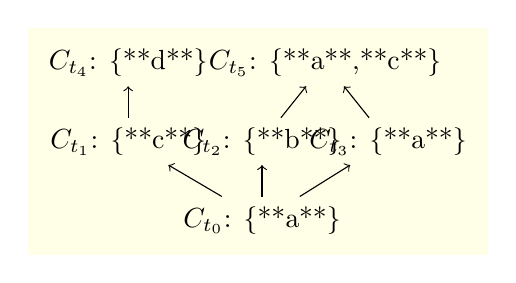
\begin{tikzpicture}[style={grow'=up,level distance=3em, sibling distance=2em}, level distance=8mm,background rectangle/.style={fill=yellow!10!white},show background rectangle]
        \node (t0) at (-0.8,0) {$C_{t_{0}}$: \{\is{**a**}\}};
        \node (t1) at (-2.5,1) {$C_{t_{1}}$: \{\is{**c**}\}};
        \node (t2) at (-0.8,1) {$C_{t_{2}}$: \{\is{**b**}\}};
        \node (t3) at (0.8,1) {$C_{t_{3}}$: \{\is{**a**}\}};
        \node (t4) at (-2.5,2) {$C_{t_{4}}$: \{\is{**d**}\}};
        \node (t5) at (0.0,2) {$C_{t_{5}}$: \{\is{**a**,**c**}\}};

        \path [->] (t0) edge node {} (t1);
        \path [->] (t0) edge node {} (t2);
        \path [->] (t0) edge node {} (t3);
        \path [->] (t3) edge node {} (t5);
        \path [->] (t1) edge node {} (t4);
        \path [->] (t2) edge node {} (t5);
      \end{tikzpicture}
      \caption{Corresponding set of collections}
      \label{fig:diamond_order}
    \end{subfigure}
    \vspace*{-3ex}
    \caption{An example stream and its collections (ordered by their time-stamps)}
    \vspace*{-2ex}
  \end{figure}
\end{frame}

\begin{frame}
  \frametitle{Sequential Composition}
  \begin{itemize}
    \item Composition
    \item Skip n
  \end{itemize}
\end{frame}

\section{Time-Aware Operators}

\begin{frame}
  \frametitle{Monotone and Productive Time-Aware Streams}
  \begin{itemize}
    \item Monotone
    \item Productive
  \end{itemize}
\end{frame}

\begin{frame}[fragile]
  \frametitle{Building Blocks: Batch Operator}

\end{frame}

\begin{frame}[fragile]
  \frametitle{Batch Operator: Soundness}

\end{frame}

\begin{frame}[fragile]
  \frametitle{Batch Operator: Completeness}
  \begin{itemize}
    \item Uses soundness of \is{batch_op}
    \item Proof by induction over n
  \end{itemize}

  \begin{tcolorbox}[ams align,colback=yellow!10!white,colframe=my_red]
    \hspace*{-0.6cm}
  \begin{array}{@{}l@{}}
    \text{\is{mono_prod lxs W --> (?i d. enat i < llength lxs \\<and> lnth lxs i = DT t d \\<and> n = Suc i) \\<or>}}
    \\
    \text{\is{n = 0 \\<and> t \\in set_t buf --> (\\<forall>t' \\in set_t buf. lfinite lxs \\<or> ?wm >= t' . WM wm \\in lset lxs) -->>}}
    \\
    \text{\is{?wm batch. DT wm batch \\in lset (produce (batch_op buf) lxs) \\<and> t \\in set_t batch \\<or>}}
    \\
    \text{\is{(\\<forall>k  \\in \{n ..< the_enat (llength lxs)\} . \\<not> (?t' >= t. lnth lxs k = WM t')) \\<and> lfinite lxs}}
  \end{array}
  \end{tcolorbox}
\end{frame}

\begin{frame}[fragile]
  \frametitle{Batch Operator: Monotone}

\end{frame}

\begin{frame}[fragile]
  \frametitle{Batch Operator: Productive}

\end{frame}

\begin{frame}[fragile]
  \frametitle{Building Blocks: Incremental Operator}

\end{frame}

\begin{frame}[fragile]
  \frametitle{Batch Operator: Soundness}

\end{frame}

\begin{frame}[fragile]
  \frametitle{Batch Operator: Completeness}

\end{frame}

\begin{frame}[fragile]
  \frametitle{Batch Operator: Monotone}

\end{frame}

\begin{frame}[fragile]
  \frametitle{Batch Operator: Productive}

\end{frame}

\begin{frame}[fragile]
  \frametitle{Compositional Reasoning}

\end{frame}

\section{Case Study}

\begin{frame}
  \frametitle{Histogram}
\end{frame}

\begin{frame}
  \frametitle{Histogram: Soundness}

\end{frame}

\begin{frame}
  \frametitle{Histogram: Completeness}
\end{frame}

\begin{frame}
  \frametitle{Histogram: Monotone}
\end{frame}

\begin{frame}
  \frametitle{Histogram: Productive}
\end{frame}

\begin{frame}
  \frametitle{Efficient Histogram}
  \begin{itemize}
    \item Foo
  \end{itemize}
\end{frame}

\begin{frame}
  \frametitle{Join}
\end{frame}

\begin{frame}
  \frametitle{Join: Soundness}
\end{frame}

\begin{frame}
  \frametitle{Join: Completeness}
\end{frame}

\begin{frame}
  \frametitle{Join: Monotone}
\end{frame}

\section{Next Steps}

\begin{frame}
  \frametitle{Next Steps}
\end{frame}

\section{Questions, comments and suggestions}

\end{document}
